\chapter{\label{cha:sts_state_of_the_art_methods}Improving State of the Art Methods}

The biggest challenge that the neural based architectures face when applied to STS tasks is the small size of datasets available to train them. As a result, in many cases the networks cannot be trained properly. Given the amount of human labour required to produce datasets for STS, it is not possible to have high quality large training datasets. As a result researches working in the field have also considered unsupervised methods for STS. Recent unsupervised approaches use pretrained word/sentence embeddings directly for the similarity task without training a neural network model on them. Such approaches have used cosine similarity on sent2vec \cite{pagliardini-etal-2018-unsupervised}, InferSent \cite{conneau-EtAl:2017:EMNLP2017}, Word Mover's Distance \cite{10.5555/3045118.3045221}, Doc2Vec \cite{10.5555/3044805.3045025} and Smooth Inverse Frequency with GloVe vectors \cite{DBLP:conf/iclr/AroraLM17}. While these approaches have produced decent results in the final rankings of shared tasks, they have also provided strong baselines for the STS task. 

This chapter explores the performance of three unsupervised STS methods - cosine similarity using average vectors, Word Mover's Distance \cite{10.5555/3045118.3045221} and cosine similarity using Smooth Inverse Frequency \cite{DBLP:conf/iclr/AroraLM17} and how to improve them using contextual word embeddings which will be explained more in Section \ref{sec:state_related}. 

We address four research questions in this chapter:

\textbf{RQ1:} Can contextual word embedding models like BERT be used to improve unsupervised STS methods?

\textbf{RQ2:} How well such an unsupervised method perform compared to other popular supervised/ unsupervised STS methods?

\textbf{RQ3:} Can the proposed unsupervised STS method be easily adopted in to different languages?

\textbf{RQ4:} How well the proposed unsupervised STS method perform in a different domain? 


The main contributions of this chapter are as follows.

\begin{enumerate}
	\item In the Related Work Section (Section \ref{sec:state_related}), we cover three unsupervised STS techniques to compute semantic similarity at the sentence level. 
	
	\item We evaluate sentence en on three English STS datasets, two non-English STS datasets and a bio-medical STS dataset which were introduced in Chapter \ref{cha:sts_introduction}.
	
	\item The code with the experiments conducted are publicly available to the community\footnote{The public GitHub repository is available on \url{https://github.com/tharindudr/simple-sentence-similarity}}.
	
	\item We published the findings in this chapter in \citet{ranasinghe-etal-2019-enhancing}.
	
\end{enumerate}

The rest of this chapter is organised as follows. Section \ref{sec:state_related} describes the three unsupervised STS methods we experimented in this section. In section \ref{sec:state_method} we present the methodology, the contextual word embeddings we used followed by the results to the English datasets comparing with the baselines. Section \ref{sec:state_languages} and Section \ref{sec:state_domains} shows how our method can be applied to different languages and domains and their results. The chapter finishes with conclusions and ideas for future research directions in unsupervised STS methods.


\section{Related Work}
\label{sec:state_related}
Given that a good STS metric is required for a variety of natural language processing fields, researchers have proposed a large number of such metrics. Before the shift of interest in neural networks, most of the proposed methods relied heavily on feature engineering. With the introduction of word embedding models, researchers focused more on neural representation for this task. 

As we mentioned before, there are two main approaches which employ neural representation models: supervised and unsupervised. Unsupervised approaches use pretrained word/sentence embeddings directly for the similarity task without training a neural network model on them while supervised approaches uses a machine learning model trained to predict the similarity using word embeddings. Since this chapter focuses on unsupervised STS methods, this section would contain the previous research done on unsupervised STS methods.


The three unsupervised STS methods explored in this chapter: Cosine similarity on average vectors, Word Mover's Distance and Cosine similarity using Smooth Inverse Frequency are the most common unsupervised methods explored in STS tasks. Apart from them, cosine similarity of the output from Infersent \cite{conneau-EtAl:2017:EMNLP2017}, sent2vec \cite{pagliardini-etal-2018-unsupervised} and doc2vec \cite{10.5555/3044805.3045025} have been used to represent the similarity between two sentences which we discuss in the next chapter. 


\subsection{Cosine Similarity on Average Vectors}
The first unsupervised STS method that we considered to estimate the semantic similarity between a pair of sentences, takes the average of the word embeddings of all words in the two sentences, and calculates the cosine similarity between the resulting embeddings. This is a common way to acquire sentence embeddings from word embeddings. Obviously, this simple baseline leaves considerable room for variation. Researches have investigated the effects of ignoring stopwords and computing an average weighted by tf-idf in particular.

\subsection{Word Mover's Distance}
The second STS state of the arts method that we have considered is Word Mover's Distance introduced by \citet{10.5555/3045118.3045221}. Word Mover's Distance uses the word embeddings of the words in two texts to measure the minimum distance that the words in one text need to ``travel'' in semantic space to reach the words in the other text as shown in Figure \ref{fig:WMD}. \citet{10.5555/3045118.3045221} shows that this is a good approach than vector averaging since this technique keeps the word vectors as it is through out the operation.

\begin{figure}[ht]
	\centering
	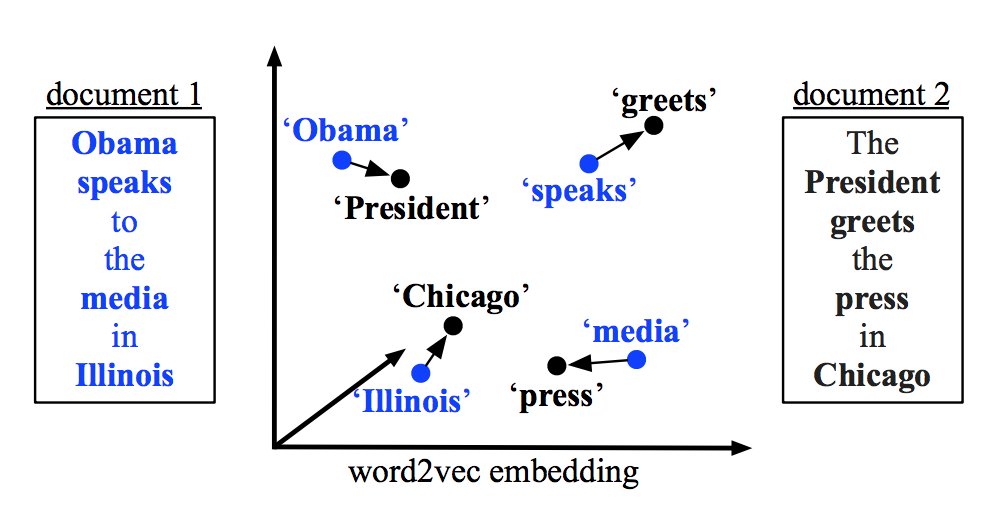
\includegraphics[scale=0.4]{figures/semantic_textual_similarity/state_of_the_art/word_movers_distance.png}
	\caption{The Word Mover's Distance between two sentences}
	\label{fig:WMD}
\end{figure}

\subsection{Cosine Similarity Using Smooth Inverse Frequency}
The third and the last unsupervised STS method we have considered is to acquire sentence embeddings using Smooth Inverse Frequency proposed by \citet{DBLP:conf/iclr/AroraLM17} and then calculate the cosine similarity between those sentence embeddings. Semantically speaking, taking the average of the word embeddings in a sentence tends to give too much weight to words that are quite irrelevant. Smooth Inverse Frequency tries to solve this problem in two steps. 

\begin{enumerate}
	\item Weighting: Smooth Inverse Frequency takes the weighted average of the word embeddings in the sentence. Every word embedding is weighted by $a\over{a + p(w)}$, where $a$ is a parameter that is typically set to 0.001 and $p(w)$ is the estimated frequency of the word in a reference corpus. 
	\item Common component removal: After that, Smooth Inverse Frequency computes the principal component of the resulting embeddings for a set of sentences. It then subtracts their projections on first principal component from these sentence embeddings. This should remove variation related to frequency and syntax that is less relevant semantically.
\end{enumerate}

As a result, Smooth Inverse Frequency downgrades unimportant words such as \emph{but, just}, etc., and keeps the information that contributes most to the semantics of the sentence. After acquiring the sentence embeddings for a pair of sentences, the cosine similarity between those two vectors were taken to represent the similarity between them. 

All of these STS methods are based on word embeddings/vectors. The main weakness of word vectors is that each word has the same unique vector regardless of the context it appears. Consider the word "play" which has several meanings, but in standard word embeddings such as GloVe \cite{pennington2014glove}, fastText \cite{mikolov-etal-2018-advances} or Word2Vec  \cite{10.5555/2999792.2999959} each instance of the word has the same representation regardless of the meaning which is used. For example the word 'bank' in two sentences - ``I am walking by the river bank'' and ``I deposited money to the bank'' would have the same embeddings which can be confusing for machine learning models. The recent introduction of contextualised word representations solved this problem by providing vectors for words considering their context too. In this way the word 'bank' in above sentences have two different embeddings. Contextual word embedding models have improved the results of many natural language processing tasks over traditional word embedding models \cite{peters-etal-2018-deep, devlin-etal-2019-bert}. However, to the best of our knowledge they have not been applied on unsupervised STS methods.

 
Therefore, we explore how the contextualised word representations can improve the above mentioned unsupervised STS methods. We will explain the neural network architectures of these contextual word embeddings in Chapter \ref{cha:sts_transformers}. For this chapter, we considered these architectures as a black box where we just feed the words to get the embeddings. We considered these contextualised word representations mainly considering the popularity they had by the time we were doing the experiments.

\begin{enumerate}
\item \textbf{ELMo\footnote{More details about ELMo can be viewed on \url{https://allennlp.org/elmo}}}
introduced by \citet{peters-etal-2018-deep} use bidirectional language model (biLM) to learn both word (e.g., syntax and semantics) and linguistic context. After pre-training, an internal state of vectors can be transferred to downstream natural language processing tasks. ELMo vectors have been successfully used in many natural language processing tasks like text classification \cite{jiang-etal-2019-team}, named entity recognition \cite{Luo2018} which motivated us to explore ELMo in unsupervised STS methods. Also, we were aware about the fact that ELMo has been pre-trained on different languages \cite{che-EtAl:2018:K18-2} and different domains \cite{jin2019probing} which will be easier when we are adopting our methodology for different languages and domains in Sections \ref{sec:state_languages} and \ref{sec:state_domains}.

\item \textbf{BERT\footnote{The GitHub repository of BERT is available on \url{https://github.com/google-research/bert}}} introduced by \citet{devlin-etal-2019-bert} might probably be the most popular contextualised word embedding model. In contrast to ELMo which uses a shallow concatenation layer \cite{devlin-etal-2019-bert}, BERT employs a deep concatenation layer. As a result BERT is considered a very powerful embedding architecture. BERT has been successfully applied in many natural language processing tasks like text classification \cite{Ranasinghe2019a}, word similarity \cite{hettiarachchi-etal-2020-brums}, named entity recognition \cite{10.1145/3394486.3403149}, question and answering \cite{yang-etal-2019-end} etc. Similar to ELMo, BERT too has been widely adopted to different languages\footnote{Information about pretrained BERT models for different languages can be found on \url{https://bertlang.unibocconi.it/}} such as Arabic \cite{antoun-etal-2020-arabert}, French \cite{martin-etal-2020-camembert}, Spanish \cite{CaneteCFP2020}, Greek \cite{10.1145/3411408.3411440} etc. and different domains such as SciBERT \cite{beltagy-etal-2019-scibert}, BioBERT \cite{10.1093/bioinformatics/btz682}, LEGAL-BERT \cite{chalkidis-etal-2020-legal} etc.  

\item \textbf{Flair\footnote{The GitHub repository of Flair is available on \url{https://github.com/flairNLP/flair}}} is another type of popular contextualised word embeddings introduced in \citet{akbik-etal-2018-contextual}. It takes a different approach by using a character level language model rather than the word level language model used in ELMo and BERT. Flair also has been used successfully in natural language processing tasks such as named entity recognition \cite{akbik-etal-2019-pooled}, part-of-speech tagging \cite{akbik-etal-2018-contextual} and has been widely adopted in to different languages and domains \cite{akbik-etal-2018-contextual,sharma2019bioflair}.

\end{enumerate}

Apart from using these contextual word embedding models individually we also considered \textbf{Stacked Embeddings} of these models together. Stacked Embeddings are obtained by concatenating different embeddings. According to \citet{akbik-etal-2018-contextual} stacking the embeddings can provide powerful embeddings to represent words. Therefore, we experimented with several combinations of Stacked Embeddings.

Even though these contextual word embedding models have shown promising results in many natural language processing tasks, to the best of our knowledge none of these contextual word representations has been applied on unsupervised STS methods.  



\section{Improving State of the Art STS Methods}
\label{sec:state_method}
As mentioned before we applied different contextual word embeddings on three unsupervised STS methods and their variants. First we experimented with English STS datasets we explained in Section \ref{sec:sts_intro_datsets}. Our implementation was based on \textit{Flair-NLP} Framework \cite{akbik-etal-2019-flair} which makes it easier to switch between different word embedding models when acquiring word embeddings. Also \textit{Flair-NLP} has their own model zoo of pre-trained models to allow researchers to use state-of-the-art NLP models in their applications. For English, all of these contextualised word embedding models come with different variants like \textit{small, large etc.}. Usually the larger models provide a better accuracy since they have been trained on a bigger dataset compared to the smaller models. However, this comes with the disadvantage that these larger models are resource-intensive than the smaller models. In order to achieve a better accuracy, we used the largest model available in each contextual word embedding models. We will describe them in the following paragraphs. 

For ELMo we used the 'original (5.5B)' pre-trained model provided in \citet{peters-etal-2018-deep} which was trained on a dataset of 5.5B tokens consisting of Wikipedia (1.9B) and all of the monolingual news crawl data from WMT\footnote{WMT: Workshop on Statistical Machine Translation is a leading conference in NLP that is being organised annually.} 2008-2012 (3.6B). \citet{peters-etal-2018-deep} mentions that ELMo original (5.5B) has slightly higher performance than other ELMo models and recommend it as a default model. Using this model we represented each word as a vector with a size of 3072 values.

For BERT we used the 'bert-large-cased' pre-trained model. Compared to the 'bert-base-cased' model, this model provided slightly better results in all the NLP tasks experimented in \citet{devlin-etal-2019-bert}. We represented each word as a 4096 lengthened vector using this model. 

As suggested in \citet{akbik-etal-2018-contextual} the recommended way to use Flair embeddings is to stack pre-trained 'news-forward' flair embeddings and pre-trained flair 'news-backward' embeddings with GloVe \cite{pennington-etal-2014-glove} word embeddings. We used the stacked model to represent each word as a 4196 lengthened vector. 

As mentioned before we also considered stacked embeddings of ELMo and BERT. For this we used pre-trained 'bert-large-uncased' model and 'original (5.5B)' pre-trained ELMo model to represent each word as a 4096 + 3072 vector.

In order to compare the results of contextualised word embeddings, we used a standard word representation model in each experiment as a baseline. In this research we used Word2vec embeddings \cite{DBLP:journals/corr/abs-1301-3781} pre-trained on Google news corpus\footnote{Pretrained Word2vec can be downloaded from \url{https://code.google.com/archive/p/word2vec/}}. We represented each word as a 300 lengthened vector using this model.

In the following list we show the performance of each unsupervised STS method with contextual word embeddings on different English STS datasets. 

\begin{enumerate}
	\item \textbf{Cosine Similarity on Average Vectors} - The first unsupervised STS method we tried to improve using contextual word embeddings is Cosine Similarity on Average Vectors which we explained on Section \ref{sec:state_related}. Table \ref{tab:sick_average_vectors} shows the results for SICK dataset, Table \ref{tab:sts_average_vectors} shows the results for STS 2017 dataset and Table \ref{tab:quora_average_vectors} shows the results for Quora Question Pairs dataset. In order to compare our results with the other systems, we conducted the experiments only on the test data of the three mentioned datasets. Since this method leaves considerable room for variation, we have investigated the following variations and reported their results in each table. 
	
	\begin{enumerate}
		\item All the word vectors were considered for averaging. Results are shown in column I of Tables \ref{tab:sick_average_vectors}, \ref{tab:sts_average_vectors} and \ref{tab:quora_average_vectors}
		
		\item All the word vectors except the vectors for stop words were considered for averaging. Column II of Tables \ref{tab:sick_average_vectors}, \ref{tab:sts_average_vectors} and \ref{tab:quora_average_vectors} shows the results. 
		
		\item All the word vectors were weighted from its tf-idf scores and considered averaging. Results are shown in column III of Tables \ref{tab:sick_average_vectors}, \ref{tab:sts_average_vectors} and \ref{tab:quora_average_vectors}
		
		\item Stop words were removed first and remaining word vectors were weighted from its tf-idf scores and considered averaging. Column IV of Tables \ref{tab:sick_average_vectors}, \ref{tab:sts_average_vectors} and \ref{tab:quora_average_vectors} shows the results.  
		
	\end{enumerate}
	
\begin{table*}[htb]
	%\footnotesize
	\centering
	\scalebox{0.95}{
		\begin{tabular}{|l|cc|cc|cc|cc|}
			
			\hline & 
			\multicolumn{2}{c|}{\textbf{I}}    & \multicolumn{2}{c|}{\textbf{II}}   & \multicolumn{2}{c|}{\textbf{III}}  &    
			\multicolumn{2}{c|}{\textbf{IV}}   \\ 
			\hline
			\multicolumn{1}{|l|}{\textbf{Model}} 
			& $\bm{\rho}$   & $\bm{\tau}$     
			& $\bm{\rho}$   & $\bm{\tau}$  
			& $\bm{\rho}$   & $\bm{\tau}$  
			& $\bm{\rho}$   & $\bm{\tau}$  
			\\ \hline
			\textit{Word2vec}                  
			& \textbf{0.730}$^{\dagger}$  & 0.624        
			& \textbf{0.714}        & 0.583    
			& \textbf{0.693}        & 0.570    
			& \textbf{0.687}        & 0.555    \\
			\textit{ELMo}                     
			& 0.669                 & 0.592         
			& 0.693                 & 0.603       
			& 0.676                 & \textbf{0.579}  
			& 0.668                 & \textbf{0.572}      \\
			\textit{Flair}                     
			& 0.646                 & 0.568         
			& 0.670                 & 0.562       
			& 0.644                 & 0.535  
			& 0.643                 & 0.531      \\
			\textit{BERT}                     
			& 0.683                 & 0.633         
			& 0.686                 & 0.606       
			& 0.557                 & 0.552  
			& 0.539                 & 0.538 \\
			\textit{ELMo $\bigoplus$ BERT}                     
			& 0.696                 & \textbf{0.634}$^{\dagger}$          
			& 0.702                 & \textbf{0.614}       
			& 0.607                 & 0.562  
			& 0.591                 & 0.551 \\
			\hline
		\end{tabular}
	}
	\caption[Results for SICK with Vector Averaging]{Results for SICK dataset with Vector Averaging. I, II, III and IV indicates the different variations as explained before. For each word embedding model, Pearson Correlation ($\bm{\rho}$) and Spearman Correlation ($\bm{\tau}$) are reported on all variations between the predicted values and the gold labels of the test set. $\bigoplus$ indicates a stacked word embedding model. Best result in each variation is marked in \textbf{Bold}. Best result from all the variations is marked with ${\dagger}$. }  
	\label{tab:sick_average_vectors}
\end{table*}

\begin{table*}[htb]
	%\footnotesize
	\centering
	\scalebox{0.95}{
		\begin{tabular}{|l|cc|cc|cc|cc|}
			
			\hline & 
			\multicolumn{2}{c|}{\textbf{I}}    & \multicolumn{2}{c|}{\textbf{II}}   & \multicolumn{2}{c|}{\textbf{III}}  &    
			\multicolumn{2}{c|}{\textbf{IV}}   \\ 
			\hline
			\multicolumn{1}{|l|}{\textbf{Model}} 
			&  $\bm{\rho}$   & $\bm{\tau}$      
			&  $\bm{\rho}$   & $\bm{\tau}$  
			&  $\bm{\rho}$   & $\bm{\tau}$  
			&  $\bm{\rho}$   & $\bm{\tau}$  
			\\ \hline
			\textit{Word2vec}                     
			& \textbf{0.625}$^{\dagger}$ & 0.583         
			& 0.609             & \textbf{0.635}       
			& \textbf{0.640}    & \textbf{0.591} 
			& \textbf{0.588}    & \textbf{0.573} \\
			\textit{ELMo}                     
			& 0.575                      & 0.574         
			& \textbf{0.618}             & 0.609       
			& 0.374                      & 0.395  
			& 0.352                      & 0.376 \\
			\textit{Flair}                     
			& 0.411                      & 0.444         
			& 0.584                      & 0.586       
			& 0.325                      & 0.374  
			& 0.336                      & 0.386 \\
			\textit{BERT}                     
			& 0.575                      & 0.574         
			& 0.555                      & 0.588       
			& 0.355                      & 0.401  
			& 0.309                      & 0.386 \\
			\textit{ELMo $\bigoplus$ BERT}                     
			& 0.600                      & \textbf{0.597}$^{\dagger}$         
			& 0.591                      & 0.608       
			& 0.391                      & 0.413  
			& 0.354                      & 0.398 \\
			\hline
		\end{tabular}
	}
	\caption[Results for STS 2017 with Vector Averaging]{Results for STS 2017 dataset with Vector Averaging. I, II, III and IV indicates the different variations as explained before. For each word embedding model, Pearson Correlation ($\bm{\rho}$) and Spearman Correlation ($\bm{\tau}$) are reported on all variations between the predicted values and the gold labels of the test set. $\bigoplus$ indicates a stacked word embedding model. Best result in each variation is marked in \textbf{Bold}. Best result from all the variations is marked with ${\dagger}$. }  
	\label{tab:sts_average_vectors}
\end{table*}

\begin{table*}[htb]
	%\footnotesize
	\centering
	\scalebox{0.95}{
		\begin{tabular}{|l|c|c|c|c|}
			
			\hline
			& \multicolumn{1}{c|}{\textbf{I}} & \multicolumn{1}{c|}{\textbf{II}}             & \multicolumn{1}{c|}{\textbf{III}}  &    
			\multicolumn{1}{c|}{\textbf{IV}} \\ 
			\hline
			\multicolumn{1}{|l|}{\textbf{Model}} & RMSE   & RMSE     &  RMSE & RMSE 
			\\ \hline
			\textit{Word2vec}  
			& \textbf{0.621}                      & \textbf{0.591}$^{\dagger}$    
			& \textbf{0.646}                      & \textbf{0.607}       \\
			\textit{ELMo}  
			& 0.629                      & 0.615    
			& 0.652                      & 0.649       \\
			\textit{Flair}  
			& 0.720                      & 0.711    
			& 0.743                      & 0.735       \\
			\textit{BERT}  
			& 0.651                      & 0.643    
			& 0.673                      & 0.662       \\
			\textit{ELMo $\bigoplus$ BERT}  
			& 0.625                      & 0.611    
			& 0.650                      & 0.647       \\	
			\hline
		\end{tabular}
	}
	\caption[Results for QUORA with Vector Averaging]{Results for QUORA dataset with Vector Averaging. I, II, III and IV indicates the different variations as explained before. For each word embedding model, Root Mean Squared Error (RMSE) is reported on all variations. $\bigoplus$ indicates a stacked word embedding model. Best result in each variation is marked in \textbf{Bold}. Best result from all the variations is marked with ${\dagger}$. }  
	\label{tab:quora_average_vectors}
\end{table*}

	From the results in Table \ref{tab:sick_average_vectors}, \ref{tab:sts_average_vectors} and \ref{tab:quora_average_vectors} there is no clear indication that contextualised word embeddings perform better than the standard word embeddings. In all the datasets considered, the best result was provided by Word2vec. 
	
	All the contextualised word embedding models we considered have more than 3000 dimensions for the word representation which is higher than the number of dimensions for the word representation we had for standard embeddings - 300. As the vector averaging model is highly dependent on the number of dimensions that a vector can have, the curse of dimensionality might be the reason for the poor performance of contextualised word embeddings in state of the art STS methods. 

	
	\item \textbf{Word Mover's Distance} - As the second unsupervised STS method we experimented with Word Mover's Distance explained on Section \ref{sec:state_related}. Similar to the average vectors, we compared having contextualised word embeddings in the place of traditional word embeddings in Word Mover's Distance. Table \ref{tab:sick_word_movers} shows the results for SICK dataset. Table \ref{tab:sts_word_movers} shows the results for STS 2017 dataset and Table \ref{tab:quora_word_movers} shows the results for Quora Questions Pairs dataset. We have investigated the effects of considering/ ignoring stop words before calculating the word mover's distance which are detailed below. 
	
	\begin{enumerate}
		\item Considering all the words to calculate the Word Mover's Distance. Results are shown in column I of Tables \ref{tab:sick_word_movers}, \ref{tab:sts_word_movers} and \ref{tab:quora_word_movers}
		\item Removing stop words before calculating the Word Mover's Distance. Column II of Tables \ref{tab:sick_word_movers}, \ref{tab:sts_word_movers} and \ref{tab:quora_word_movers} shows the results. 
	\end{enumerate} 
	
	

\begin{table*}[htb]
	%\footnotesize
	\centering
	\scalebox{0.95}{
		\begin{tabular}{|l|cc|cc|}
			
			\hline & 
			\multicolumn{2}{c|}{\textbf{I}}    & \multicolumn{2}{c|}{\textbf{II}}   \\ 
			\hline
			\multicolumn{1}{|l|}{\textbf{Model}} 
			& $\bm{\rho}$   & $\bm{\tau}$     
			& $\bm{\rho}$   & $\bm{\tau}$  
			\\ \hline
			\textit{Word2vec}                  
			& \textbf{0.730}$^{\dagger}$  & 0.624        
			& \textbf{0.714}        & 0.583   \\
			\textit{ELMo}                     
			& 0.669                 & 0.592         
			& 0.693                 & 0.603    \\
			\textit{Flair}                     
			& 0.646                 & 0.568         
			& 0.670                 & 0.562    \\
			\textit{BERT}                     
			& 0.683                 & 0.633         
			& 0.686                 & 0.606  \\
			\textit{ELMo $\bigoplus$ BERT}                     
			& 0.696                 & \textbf{0.634}$^{\dagger}$          
			& 0.702                 & \textbf{0.614}  \\
			\hline
		\end{tabular}
	}
	\caption[Results for SICK with Word Mover's Distance]{Results for SICK dataset with Word Mover's Distance. I and II indicates the different variations as explained before. For each word embedding model, Pearson Correlation ($\bm{\rho}$) and Spearman Correlation ($\bm{\tau}$) are reported on all variations between the predicted values and the gold labels of the test set. $\bigoplus$ indicates a stacked word embedding model. Best result in each variation is marked in \textbf{Bold}. Best result from all the variations is marked with ${\dagger}$. }  
	\label{tab:sick_word_movers}
\end{table*}

\begin{table*}[htb]
	%\footnotesize
	\centering
	\scalebox{0.95}{
		\begin{tabular}{|l|cc|cc|}
			
			\hline & 
			\multicolumn{2}{c|}{\textbf{I}}    & \multicolumn{2}{c|}{\textbf{II}}   \\ 
			\hline
			\multicolumn{1}{|l|}{\textbf{Model}} 
			&  $\bm{\rho}$   & $\bm{\tau}$      
			&  $\bm{\rho}$   & $\bm{\tau}$   
			\\ \hline
			\textit{Word2vec}                     
			& \textbf{0.625}$^{\dagger}$ & 0.583         
			& 0.609             & \textbf{0.635} \\
			\textit{ELMo}                     
			& 0.575                      & 0.574         
			& \textbf{0.618}             & 0.609 \\
			\textit{Flair}                     
			& 0.411                      & 0.444         
			& 0.584                      & 0.586\\
			\textit{BERT}                     
			& 0.575                      & 0.574         
			& 0.555                      & 0.588 \\
			\textit{ELMo $\bigoplus$ BERT}                     
			& 0.600                      & \textbf{0.597}$^{\dagger}$   & 0.591                      & 0.608  \\
			\hline
		\end{tabular}
	}
	\caption[Results for STS 2017 with Word Mover's Distance]{Results for STS 2017 dataset with Word Mover's Distance. I and II indicate the different variations as explained before. For each word embedding model, Pearson Correlation ($\bm{\rho}$) and Spearman Correlation ($\bm{\tau}$) are reported on all variations between the predicted values and the gold labels of the test set. $\bigoplus$ indicates a stacked word embedding model. Best result in each variation is marked in \textbf{Bold}. Best result from all the variations is marked with ${\dagger}$. }  
	\label{tab:sts_word_movers}
\end{table*}

\begin{table*}[htb]
	%\footnotesize
	\centering
	\scalebox{0.95}{
		\begin{tabular}{|l|c|c|}
			
			\hline
			& \multicolumn{1}{c|}{\textbf{I}} & \multicolumn{1}{c|}{\textbf{II}}  \\ 
			\hline
			\multicolumn{1}{|l|}{\textbf{Model}} & RMSE   & RMSE     
			\\ \hline
			\textit{Word2vec}  
			& \textbf{0.621}                      & \textbf{0.591}$^{\dagger}$ \\
			\textit{ELMo}  
			& 0.629                      & 0.615      \\
			\textit{Flair}  
			& 0.720                      & 0.711       \\
			\textit{BERT}  
			& 0.651                      & 0.643     \\
			\textit{ELMo $\bigoplus$ BERT}  
			& 0.625                      & 0.611      \\	
			\hline
		\end{tabular}
	}
	\caption[Results for QUORA with Word Mover's Distance]{Results for QUORA dataset with Word Mover's Distance. I and II indicate the different variations as explained before. For each word embedding model, Root Mean Squared Error (RMSE) is reported on all variations. $\bigoplus$ indicates a stacked word embedding model. Best result in each variation is marked in \textbf{Bold}. Best result from all the variations is marked with ${\dagger}$. }  
	\label{tab:quora_word_movers}
\end{table*}

As depicted in table  contextualised word representations could not improve Word Mover's method too over standard word representations. Even though, ELMo $\bigoplus$ BERT model outperforms Word2vec in SICK and STS 2017 dataset with regard to Spearman Correlation ($\bm{\tau}$) there is no clear indication that contextual word representations would outperform standard word representations in Word Mover's method. Since the travelling distance is dependent on number of dimensions, the curse of dimensionality might be the reason for the poor performance of contextualised word representations in this scenario too.


\item \textbf{Smooth Inverse Frequency} As the third and the final unsupervised STS method we experimented with Smooth Inverse Frequency explained on Section \ref{sec:state_related}.  Similar to the previous STS methods, we compared having contextualised word embeddings in the place of traditional word embeddings in Smooth Inverse Frequency method. Since the Smooth Inverse Frequency method takes care of stop words, we did not consider any variations that we experimented with previous STS methods. Table \ref{tab:sick_smooth_inverse} shows the results for SICK dataset. Table \ref{tab:sts_smooth_inverse} shows the results for STS 2017 dataset and Table \ref{tab:quora_smooth_inverse} shows the results for Quora Questions Pairs dataset.


\begin{table*}[htb]
	%\footnotesize
	\centering
	\scalebox{0.95}{
		\begin{tabular}{|l|cc|}
			\hline
			\textbf{Model} & $\bm{\rho}$   & $\bm{\tau}$     
			\\ \hline
			\textit{Word2vec}                  
			& 0.734 & 0.632  \\
			\textit{ELMo}                     
			& 0.740 & 0.654   \\
			\textit{Flair}                     
			& 0.731 & 0.634  \\
			\textit{BERT}                     
			& 0.746 & 0.661  \\
			\textit{ELMo $\bigoplus$ BERT}                     
			& 0.753$^{\dagger}$  & 0.669$^{\dagger}$       \\
			\hline
		\end{tabular}
	}
	\caption[Results for SICK with Smooth Inverse Frequency]{Results for SICK dataset with Smooth Inverse Frequency. For each word embedding model, Pearson Correlation ($\bm{\rho}$) and Spearman Correlation ($\bm{\tau}$) are reported between the predicted values and the gold labels of the test set. $\bigoplus$ indicates a stacked word embedding model. Best result from all the variations is marked with ${\dagger}$. }  
	\label{tab:sick_smooth_inverse}
\end{table*}


\begin{table*}[htb]
	%\footnotesize
	\centering
	\scalebox{0.95}{
		\begin{tabular}{|l|cc|}
			\hline
			\textbf{Model} & $\bm{\rho}$   & $\bm{\tau}$     
			\\ \hline
		\textit{Word2vec}                  
		& 0.638 & 0.601  \\
		\textit{ELMo}                     
		& 0.641 & 0.609   \\
		\textit{Flair}                     
		& 0.639 & 0.606  \\
		\textit{BERT}                     
		& 0.650 & 0.612  \\
		\textit{ELMo $\bigoplus$ BERT}                     
		& 0.654$^{\dagger}$  & 0.616$^{\dagger}$       \\
		\hline
		\end{tabular}
	}
	\caption[Results for STS 2017 with Smooth Inverse Frequency]{Results for STS 2017 dataset with Smooth Inverse Frequency. For each word embedding model, Pearson Correlation ($\bm{\rho}$) and Spearman Correlation ($\bm{\tau}$) are reported between the predicted values and the gold labels of the test set. $\bigoplus$ indicates a stacked word embedding model. Best result from all the variations is marked with ${\dagger}$. }  
	\label{tab:sts_smooth_inverse}
\end{table*}


\begin{table*}[htb]
	%\footnotesize
	\centering
	\scalebox{0.95}{
		\begin{tabular}{|l|c|}
			\hline
			\textbf{Model} & RMSE     
			\\ \hline
			\textit{Word2vec}                  
			& 0.599 \\
			\textit{ELMo}                     
			& 0.585   \\
			\textit{Flair}                     
			& 0.589  \\
			\textit{BERT}                     
			& 0.572   \\
			\textit{ELMo $\bigoplus$ BERT}                     
			& 0.566$^{\dagger}$    \\
			\hline
		\end{tabular}
	}
	\caption[Results for QUORA with Smooth Inverse Frequency]{Results for QUORA dataset with Smooth Inverse Frequency. For each word embedding model, Root Mean Squared Error (RMSE) is reported. $\bigoplus$ indicates a stacked word embedding model. Best result is marked with ${\dagger}$.}  
	\label{tab:quora_smooth_inverse}
\end{table*}


As can be seen in the results, unlike the previous unsupervised STS methods, contextualised word embeddings improved the results in Smooth Inverse Frequency method compared to the standard word embeddings in all the three datasets considered. It can be observed that Smooth Inverse Frequency method is less sensitive to the number of dimensions in the word embedding model as it has a common component removal step and due to this reason, contextualised word embedding models does not suffer the \textit{Curse of dimensionality} \cite{10.1145/276698.276876} with Smooth Inverse Frequency. In all of the datasets, the stacked embedding model of ELMo and BERT (ELMo $\bigoplus$ BERT) performed best. Further evaluating, from all the unsupervised STS methods we experimented including Vector Averaging and Word Movers Distance too, ELMo $\bigoplus$ BERT with the Smooth Inverse Frequency method provided the best results. With these observations, we address our \textit{RQ1}, contextualised embeddings can be used to improve the unsupervised STS methods. Even though the contextual word embedding models did not improve the results in Vector Averaging and Word Movers Distance, there was clear improvement when they were applied on Smooth Inverse Frequency. 

With regard to our \textit{RQ2: How well the proposed unsupervised STS method performs when compared to various other STS methods?}, we compared our best results of the SICK dataset to the results in the SemEval 2014 Task 1 \cite{marelli-etal-2014-semeval} which was the original task that the SICK dataset was initiated as we mentioned before. Our unsupervised method had 0.753 Pearson correlation score, whilst the best result in the competition had 0.828 Pearson correlation \cite{marelli-etal-2014-semeval}. Our approach would be ranked on the ninth position from the top results out of 18 participants, and it is the best unsupervised STS method among the results \cite{marelli-etal-2014-semeval}. Our method even outperformed systems that rely on additional feature generation (e.g. dependency parses) or data augmentation schemes. For example, our method is just above the UoW system which relied on 20 linguistics features fed in to a Support Vector Machine and obtained a 0.714 Pearson correlation \cite{gupta-etal-2014-uow}. Compared to these complex approaches our simple unsupervised approach provides a strong baseline to STS tasks. This answers our \textit{RQ2}, that the proposed unsupervised STS method is competitive with the other supervised and unsupervised STS methods. 

\end{enumerate}


\section{Portability to Other Languages}
\label{sec:state_languages}
Our \textbf{RQ3} targets the multilinguality aspect of the proposed approach; \textit{How well the proposed unsupervised STS method performs in different languages?}. To answer this, we evaluated our method in Arabic STS and Spanish STS datasets that were introduced in Chapter \ref{cha:introduction}. Our approach has the advantage that it does not rely on language dependent features and it does not need a training set as the approach is unsupervised. As a result, the approach is easily portable to other languages given the availability of ELMo and BERT models in that particular language. 

As the contextual word embedding models, for ELMo embeddings, we used the Arabic and Spanish Elmo models released by \citet{che-EtAl:2018:K18-2}. \citet{che-EtAl:2018:K18-2} have trained ELMo models for 44 languages including Arabic and Spanish using the same hyperparameter settings as \citet{peters-etal-2018-deep} on Common Crawl and a Wikipedia dump of each language\footnote{The GitHub repository for the ELMo for many languages project is available on \url{https://github.com/HIT-SCIR/ELMoForManyLangs}}. The models are hosted in NLPL Vectors Repository \cite{fares-etal-2017-word}\footnote{More information on the NLPL Vectors Repository is available on \url{http://wiki.nlpl.eu/index.php/Vectors/home}}. As for BERT we used the "BERT-Base, Multilingual Cased" model \cite{devlin-etal-2019-bert} which has been built on the top 100 languages with the largest Wikipedias that includes Arabic and Spanish languages too. Similar to the English experiments, we conducted the experiments through the \textit{Flair-NLP} Framework \cite{akbik-etal-2019-flair}. In order to compare the results, as traditional word embeddings,  we used AraVec \cite{SOLIMAN2017256} \footnote{AraVec has been trained on Arabic Wikipedia articles. The models are available on \url{https://github.com/bakrianoo/aravec}} for Arabic and Spanish 3B words Word2Vec Embeddings \cite{doi:10.1177/1550147718811827}\footnote{Spanish 3B words Word2Vec Embeddings have been trained on Spanish news articles, Wikipedia articles and Spanish Boletín Oficial del Estado (BOE; English: Official State Gazette). The model is available on \url{https://github.com/aitoralmeida/spanish_word2vec}} for Spanish.

Similar to the English datasets, from the unsupervised STS methods we considered, Smooth Inverse Frequency with ELMo and BERT stacked embeddings gave the best results for both Arabic and Spanish datasets. For Arabic our approach had 0.624 Pearson correlation whilst the best result \cite{wu-etal-2017-bit} in the competition had 0.754 Pearson correlation \cite{cer-etal-2017-semeval}. Our approach would rank eighteenth out of 49 teams in the final results. Similar to English, our approach has the best result for an unsupervised method and surpasses other complex supervised models. For example \citet{kohail-etal-2017-sts} proposes a supervised approach, which combines dependency graph similarity and coverage features with lexical similarity measures using regression methods and scored only 0.610 Pearson correlation. This shows that the proposed unsupervised STS method outperforms this supervised STS method.


For Spanish, our approach had 0.712 Pearson correlation whilst the best result \cite{tian-etal-2017-ecnu} in the competition had 0.855 Pearson correlation \cite{cer-etal-2017-semeval}. Our approach would rank sixteenth out of 46 teams in the final results, which is the best result for an unsupervised approach. As with the English model, this one also surpasses other complex supervised models. For example \citet{barrow-peskov-2017-umdeep} uses a supervised machine learning algorithm with word embeddings and scored only 0.516 Pearson correlation. Our fairly simple unsupervised approach outperform this supervised method by a large margin. 

These findings answer our \textit{RQ3}; the proposed unsupervised STS method can be successfully applied to other languages and it is very competitive even with the supervised methods. 


\section{Portability to Other Domains}
\label{sec:state_domains}
In order to answer our \textit{RQ4}; how well the proposed unsupervised STS method can be applied in different domains, we evaluated our method on Bio-medical STS dataset explained in \ref{cha:sts_introduction}. As we mentioned before Bio-medical STS dataset does not have a training set. Therefore, only the unsupervised approaches can be applied on this dataset which provides an ideal opportunity for the STS method we introduced in this Chapter. 

For the experiments, as the contextual word embedding models, we used BioELMo \cite{jin2019probing}\footnote{BioELMo is the biomedical version of ELMo, pre-trained on PubMed abstracts. The model is available on \url{https://github.com/Andy-jqa/bioelmo}}, BioBERT \cite{10.1093/bioinformatics/btz682}\footnote{BioBERT has trained BERT on PubMed abstracts. The model is available on \url{https://github.com/dmis-lab/biobert}} and BioFLAIR \cite{sharma2019bioflair}\footnote{BioFLAIR is FLAIR embeddings trained on PubMed abstracts. The model is available on \url{https://github.com/shreyashub/BioFLAIR}}. Additionally, to compare the performance with standard word embeddings, we used BioWordVec \cite{Zhang2019}\footnote{BioWordVec has trained word2vec on a combination of PubMed and PMC texts. The model is availble on \url{https://bio.nlplab.org/}}. Same as English and multilingual experiments, Smooth Inverse Frequency with ELMo and BERT stacked embeddings performed best with this dataset too. It had 0.708 Pearson correlation, whilst the best performing method had 0.836 Pearson correlation. This would rank our approach seventh out of 22 teams in the final results of the task \cite{10.1093/bioinformatics/btx238}.

It should be also noted that it outperforms many complex methods that sometimes uses external tools too. As an example, the UBSM-Path approach is based ontology based similarity which uses METAMAP \cite{Aronson2001} for extracting medical concepts from text and our simple unsupervised approach outperform them by a significant margin. UBSM-Path only has 0.651 Pearson correlation and compared to that our simple STS method based on contextual embeddings outperform them. 

This answers our fourth and the final \textit{RQ}; the proposed unsupervised STS method can be successfully applied in to other domains and it is very competitive with the available STS methods. 



\section{Conclusions}
\label{sec:state_conclusions}

This chapter experimented three unsupervised STS methods namely cosine similarity using average vectors, Word Mover's Distance and cosine similarity using Smooth Inverse Frequency with contextualised word embeddings for calculating semantic similarity between pairs of texts and compared them with other unsupervised/ supervised approaches. Contextualised word embeddings could not improve cosine similarity using average vectors and Word Mover's Distance methods, but the results when using Smooth Inverse Frequency method were improved significantly with contextualised word embeddings, instead of standard word embeddings. Further more we learned that stacking ELMo and BERT provides a strong word representation rather than individual representations of ELMo and BERT. The results indicated that calculating cosine similarity using Smooth Inverse Frequency with stacked embeddings of ELMo and BERT is the best unsupervised method from the available approaches. Also, our approach finished on the top half of the final results list in the SICK dataset surpassing many complex and supervised approaches. 

Our approach was also applied in the Arabic, Spanish and Bio-medical STS tasks, where our simple unsupervised method finished on the top half of the final result list in all the cases outperforming many supervised/ unsupervised STS methods. Therefore, given our results we can safely assume that regardless of the language or the domain cosine similarity using Smooth Inverse Frequency with stacked embeddings of ELMo and BERT will provide a simple but strong unsupervised method for STS tasks. 

Contextual word embedding models are getting popular day by day due to their superior performance compared to standard word embedding models. Contextual word embedding models are available even in low resource languages like Assamese \cite{kakwani-etal-2020-indicnlpsuite}, Hebrew \cite{chriqui2021hebert}, Odia \cite{kakwani-etal-2020-indicnlpsuite}, Yoruba \cite{alabi-etal-2020-massive}, Twi \cite{alabi-etal-2020-massive} etc. Very soon, contextual word embedding models would be available in all the languages where  standard word embedding models available. Therefore, we can conclude that the unsupervised STS method we introduced in this chapter will be beneficial to many languages and domains. 

As future work, the experiments can be extended in to other BERT like contextual word embedding models such as XLNet \cite{yang2019xlnet}, RoBERTa \cite{liu2019roberta}, SpanBERT \cite{joshi-etal-2020-spanbert} etc. One drawback of using Contextual word embedding models is that most of the pretrained models only support 512 maximum number of tokens which would be problematic when encoding longer sequences. Therefore, STS with long sequences can be explored with recently released contextual word embedding models like Longformer \cite{beltagy2020}  and Big Bird \cite{zaheer2021} that supports encoding longer sequences than 512 maximum number of tokens. Taking advantage from the fact that this method is unsupervised and does not need a training dataset, it can further expanded in to many languages and domains as future work.   

